\section{Experiments}
\subsection{Experiment on syntatic data}
Throughout syntactical experiments, we aim at validating our main results,
which are stated at Lemma \ref{lemma:bound_on_u}. In this setting, we have to able to 
Assume the vector $\x \in \R^d$ is drawn from Gaussian distribution $N(0,\Sigma_{d \times d})$ and we are given noisy observation of a linear model $y = \langle \x, \w^* \rangle + \epsilon$, where $\epsilon$ is a
Gaussian noise $N(0,\sigma^2)$. Let $\mu$ denote the minimum eigenvalue of the
covariance matrix $\Sigma$.
We are given $n$ observation of this model i.e.
 $\T_n = \{ 
(\x_i,y_i)\}_{i=1}^n$. The empirical loss function is 
\begin{equation*}
	\risk_n(\w) = \frac{1}{n} \sum_{i=1}^n \left(\langle \x_i, \w\rangle -
	y_i\right)^2
\end{equation*}
The Hessian matrix of the above function is the empirical covariance matrix
$X_n^T X_n$.
Let the matrix $X_n$ is row-wise arrange of input vectors $x_i$s. Then
Hessian matrix of the above risk is $\Sigma_n = X_n^T X_n$. When $n \gg d$, the
matrix $\Sigma_n$ converges to $\Sigma$. Therefore, we can assume the
empirical function is also $\mu$-strongly convex. Furthermore, the Lipschitz
constant $L$ is the maximum norm of the data points. It is not difficult to
show that $\bound(n) = \bigO(\frac{1}{n})$ in this case.
\todo[inline]{ I have to prove this }
The proposed upper-bound of the convergence to ERM, which is proved at Lemma
\ref{lemma:bound_on_u}, has two main parts: the condition number dependent part $(\frac{\kappa}{n})^2$, the
generalization bound $\bound(n)$ which is independent of the condition number
$\kappa$. In the first experiment, we set the condition number $\kappa =
\sqrt{n}$. To this end, we use a diagonal matrix
$\Sigma$ with decreasing diagonal elements in a way that the largest diagonal
element is 1 and the smallest one is $\frac{1}{\sqrt{n}}$. This covariance
matrix yields us the desired condition number i.e. $\kappa = \sqrt{n}$.
According to the Lemma \ref{lemma:bound_on_u}, the upper-bound of $\U(n,n)$ is
$\bigO(n)$, as the following simple calculation shows: 
\begin{equation*}
	\U(n,n) \leq (\frac{\sqrt{n}}{n})^2 + \bound(n) = \bigO(\frac{1}{n})
\end{equation*}
To test this upper-bound, we run saga on different size of data sets for one
pass. We used the suggested sample size schedule, which is suggest at Lemma
\ref{lemma:bound_on_u}. Since, the empirical sub-optimality is $\bigO(1/n)$, we
expect that the $\log$-$\log$ plot of sub-optimality has slope less than one. On
contrary, when $\kappa = n^{\frac{3}{4}}$, the term $(\frac{\kappa}{n})^2$ is the
dominating term of the proposed upper-bound. In this case, the $\U(n,n)$ is
bounded by $\bigO(\frac{1}{\sqrt{n}})$. Consequently, $\log$-$\log$ plot of
sub-optimality vs the sample size should have a slope less than $\frac{1}{2}$.
Our experimental results confirm these theoretical results, as Figure \ref{fig:slopes}
illustrates. We have to mention that the variance of noise in our is $\sigma^2
= 0.01$.
\subsection{Experiments on Real Datasets}
The experiments on real datasets will compare performance of adaptive SAGA with
the state of the art methods.
\todo[inline]{ We need more methods to compare with. Which methods do you
suggest?} The selected dataset is ``ijcnn1'' from SVMLIB
 dataset collection \cite{REF08a}. This dataset contains 49990 training points
 with 22 features from two classes. Logistic loss is used in experiment and with
 use regularization factor $\lambda = \frac{1}{\sqrt{n}} =
 \frac{1}{\sqrt{49990}}$. We have tried two possible step size value suggested
 value $\eta = \frac{1}{3(L+\mu n )}$ and $\eta = \frac{1}{3L}$ suggested by
 the original algorithm \cite{defazio2014saga}. As Figures \ref{fig:ijcnn1} and 
 \ref{fig:ijcnn1_large} illustrate adaptive SAGA outperforms the saga and sgd. 
 \todo[inline]{
 I can not explain the difference between two plots.}
 Here, we use decreasing step size $\eta_t = \frac{\gamma}{\gamma+\mu t}$, where
 we search for a better choice of $\gamma$ parameter (the final value is $\gamma
 = 0.1$) as paper \cite{bottou2010large} suggests. 
 We also uses a dataset with larger number of features i.e. w8a from the SVM
 libaray. Our method outperforms on this dataset as well \ref{fig:wa}. Note that
 the $ADAPTDoubling$ method denotes adaptive doubling sample size strategy. The
 result on a larger dataset is covetype, which is represented at Figure
 \ref{fig:covtype}, confirms the advantages of our method. 
 \begin{figure}
\center
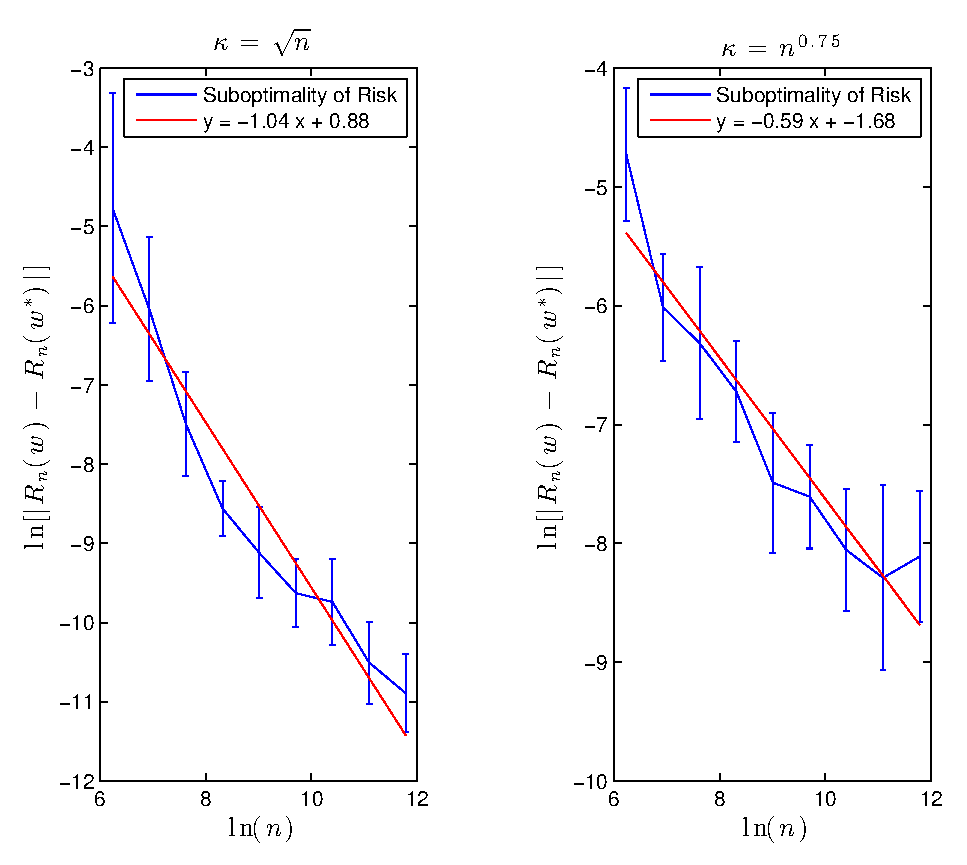
\includegraphics[width=0.8\textwidth]{slopes} 
\caption{The synatic }
\label{fig:slopes}
\end{figure}

 \begin{figure}
\center
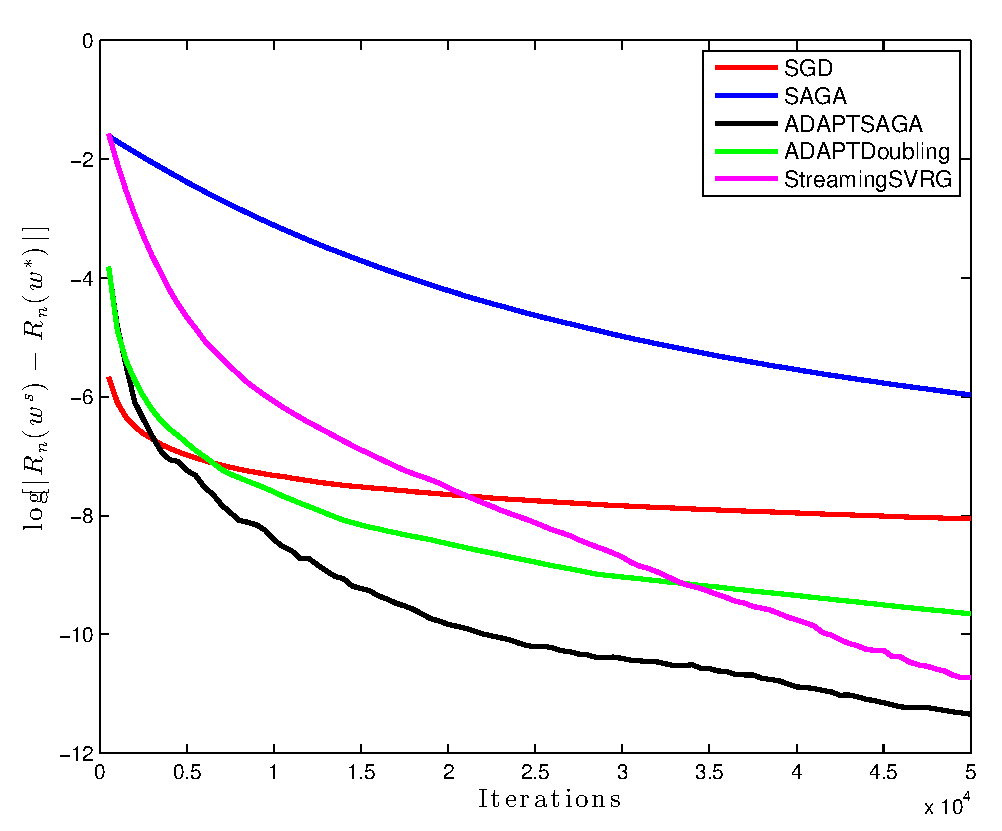
\includegraphics[width=0.5\textwidth]{ijcnn1} 
\caption{Test on ijcnn1 with step size $\eta = \frac{1}{3(\mu n + L)}$}
\label{fig:ijcnn1}
\end{figure}
\begin{figure}
\center
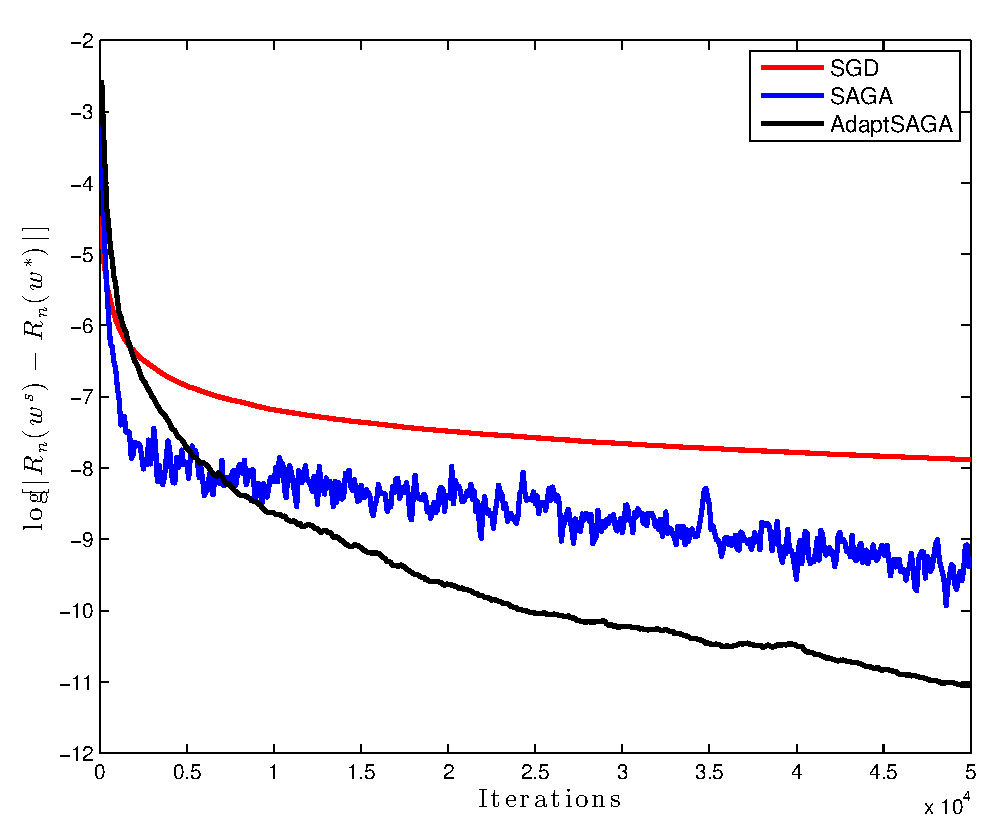
\includegraphics[width=0.5\textwidth]{ijcnn1_largestepsize} 
\caption{Test on ijcnn1 with step size $\eta = \frac{1}{3L}$}
\label{fig:ijcnn1_large}
\end{figure}
\begin{figure}
\center
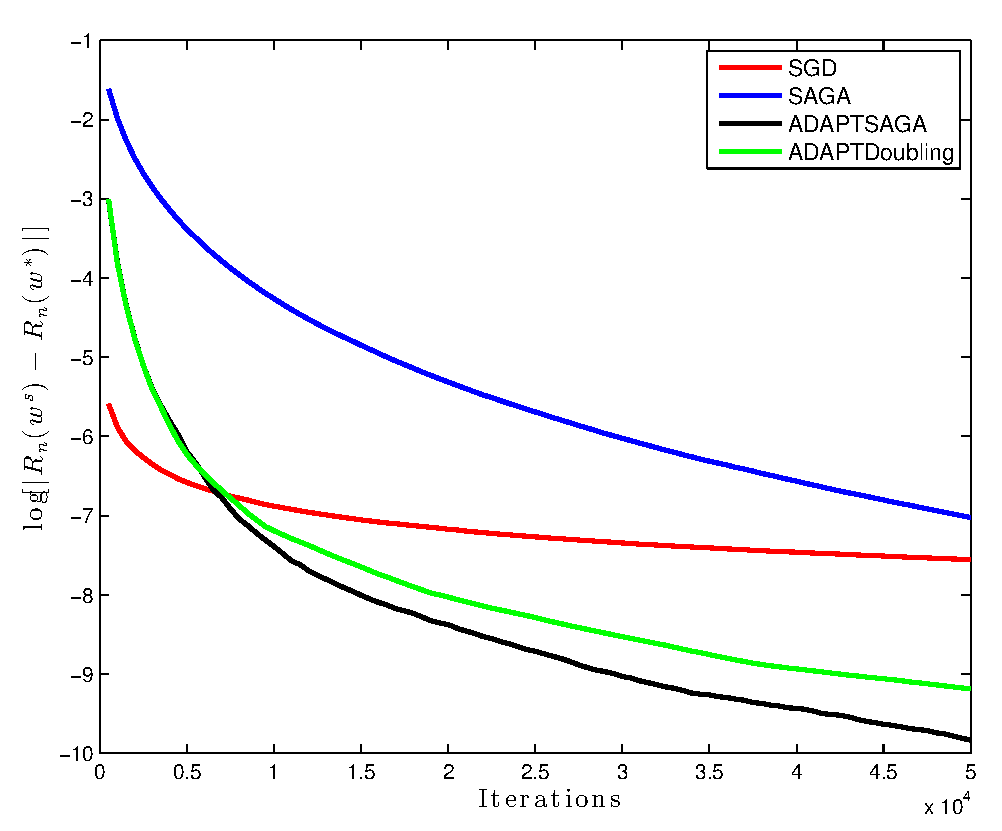
\includegraphics[width=0.5\textwidth]{wa} 
\caption{w8a dataset with $n = 49,749, d = 300$}
\label{fig:wa}
\end{figure}
\begin{figure}
\center
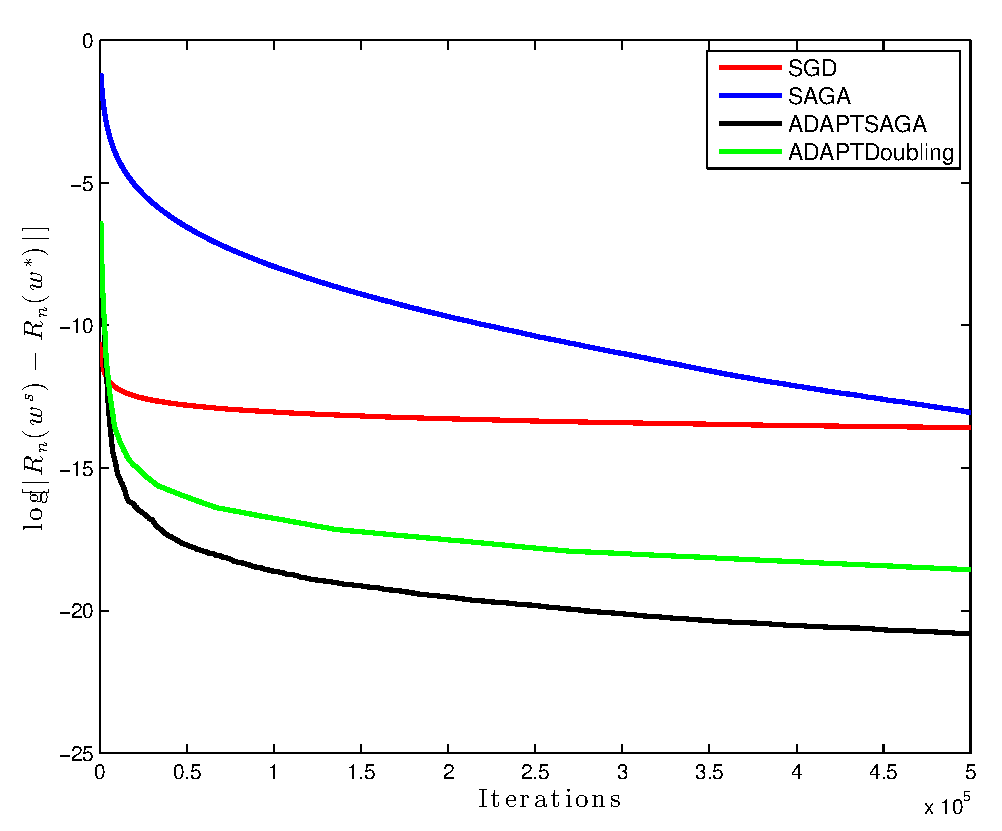
\includegraphics[width=0.5\textwidth]{covtype} 
\caption{w8a dataset with $n = 581,012, d = 54$}
\label{fig:covtype}
\end{figure}


